\chapter{Results and discussion}

\label{Chapter6}

%\lhead{Chapter 6. \emph{Results and discussion}}

%----------------------------------------------------------------------------------------
%	INTRO
%----------------------------------------------------------------------------------------
In this chapter I will present the obtained results along with little reflexions. This chapter will also be strongly correlated with the initial objectives and how they have been carried out.

The tests were done at T\`{a}nger building that belongs to the Pompeu Fabra University. In this edifice, there are a lot of Wi-Fi networks which also operate in the 2.4 GHz band, apart from wireless mesh network nodes and concrete walls (which are known to pose serious problems to this particular ISM band).

Under this environmental conditions, I set up a network whose nodes had a maximum range of 25m, half of the range indicated by the datasheet provided by Digi\footnote{\url{ftp://ftp1.digi.com/support/documentation/90000866_A.pdf}}, probably caused by spectrum saturation.

The tests were carried out with the two possible sensor nodes, which transmitted some environmental factors. A picture of one deployed node is displayed below (figure \ref{fig:arduinoventana}). Despite the messy appearance, it took ten minutes to load the sketch on the Arduino, configure the XBee\textregistered{} and wire cables and sensors. More precisely, they were measuring temperature, relative humidity and noise levels.

\begin{figure}[htbp]
    \centering
        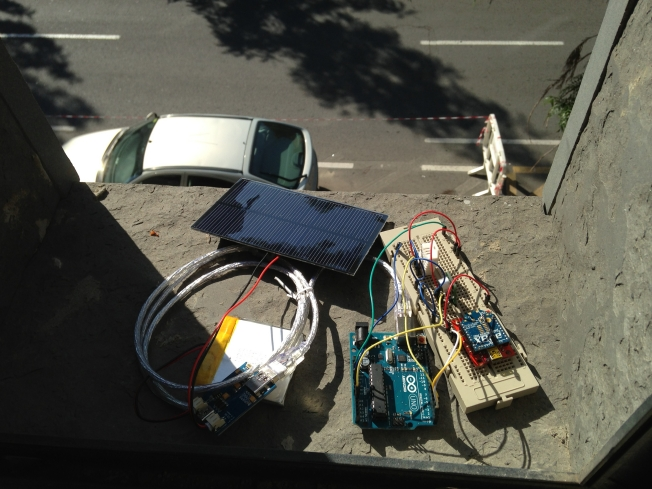
\includegraphics[scale=0.12,angle=180]{./Figures/arduinoventana.jpg}
        \rule{35em}{0.5pt}
    \caption[Real-life Arduino node]{An actual Arduino node measuring environmental factors.}
    \label{fig:arduinoventana}
\end{figure}

Then, two other nodes were transmitting at the same moment. Those were two standalone XBee\textregistered{} nodes, depicted in figure \ref{fig:noxo}. With the help of the Emartee mini sound sensor (subsection \ref{sub:sound}) and the TI LM35 (\ref{sub:lm35}) they measured noise levels and temperature. Although measured factors are somehow redundant, they served as a proof of concept of the system.

\begin{figure}[htbp]
    \centering
        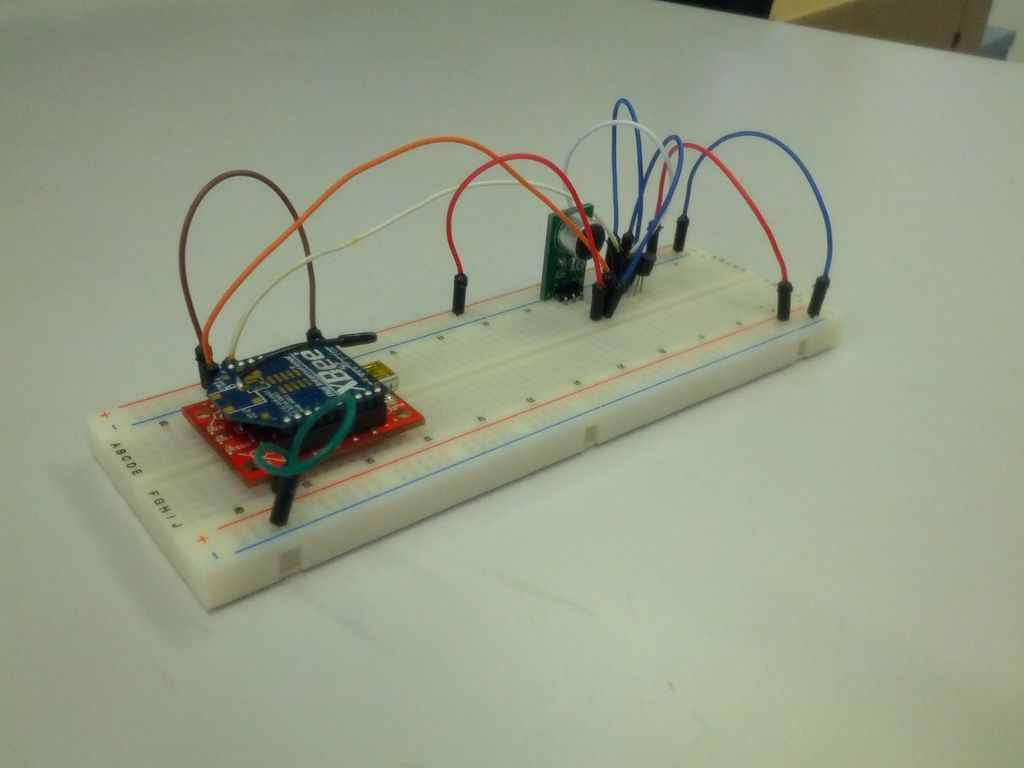
\includegraphics[scale=0.4]{./Figures/noxo.jpg}
        \rule{35em}{0.5pt}
    \caption[An actual standalone XBee\textregistered{} node]{Standalone XBee\textregistered{} measuring temperature and noise levels.}
    \label{fig:noxo}
\end{figure}

Sadly, due to lack of opportunities, no external organizations were able to test this network.


Putting aside the medium restraints of the physical medium the protocol uses, the main result of this project can be appreciated on figure \ref{fig:datos_subidos}. There, gathered data can be seen in the visualization tools that Xively provides.

\begin{figure}[htbp]
    \centering
        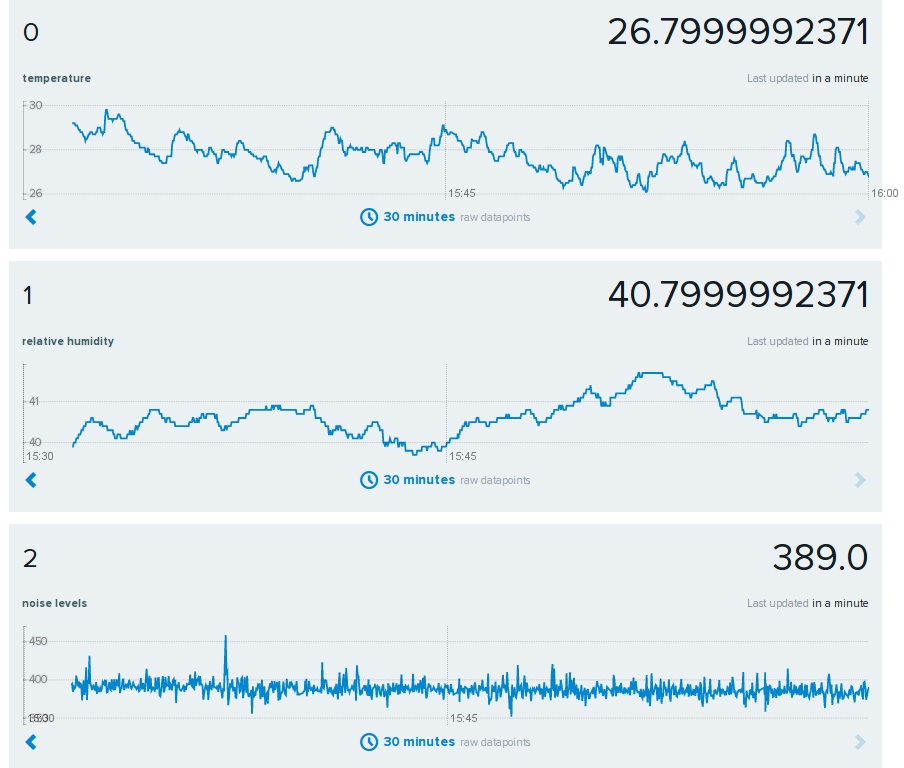
\includegraphics[scale=0.4]{./Figures/xivelyup.png}
        \rule{35em}{0.5pt}
    \caption[Data uploaded to Xively]{How data is viewed in Xively (\url{http://xively.com)}}
    \label{fig:datos_subidos}
\end{figure}

When the sink script is running, the following output is presented through \texttt{stdout} (figure \ref{fig:stdout}). That is, the original sender of the packet as well as its content.

\begin{figure}[htbp]
    \centering
        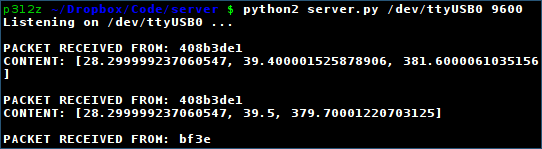
\includegraphics[scale=0.6]{./Figures/terminal.png}
        \rule{35em}{0.5pt}
    \caption[Output of the daemon]{Output of the script running.}
    \label{fig:stdout}
\end{figure}
